\documentclass[a4paper, 12p]{article}
\usepackage{graphicx}
\usepackage{hyperref}
\usepackage{enumitem}
\usepackage{csquotes}
\usepackage[T1]{fontenc}
\usepackage{caption}
\usepackage{booktabs}
\usepackage{xcolor}
\usepackage{float}
\usepackage{longtable}
\usepackage{tasks}
\usepackage{tabularx}
\usepackage{titlesec}


\titleformat{\paragraph}
{\normalfont\normalsize\bfseries}{\theparagraph}{1em}{}
\titlespacing*{\paragraph}
{0pt}{3.25ex plus 1ex minus .2ex}{1.5ex plus .2ex}
\setlength {\marginparwidth }{2cm}
\begin{document}
\begin{titlepage}
    \centering
    {\scshape\large AY 2021/2022 \par}
    \vfill
    
\includegraphics[width=100pt]{images/logo-polimi-new.pdf}\par\vspace{1cm}
    {\scshape\LARGE Politecnico di Milano \par}
    \vspace{1.5cm}
    {\huge\bfseries SMBUD 2021 - Project work\@ \\ delivery 1  \par}
    
    \vspace{1.5cm}
    {\large \textbf{Group 20} \par
    
    \begin{center}
        
         
        {\begin{tabular}{l l }
        Margherita & Musumeci \\
        Matteo & Nunziante \\
        Piero & Rendina \\
        Andrea & Sanchini \\
        Enrico & Zuccolotto \\
        \end{tabular}}
        
    \end{center}
    }
    \vfill
    \begin{center}
        {\large \textbf{Professor}\par
            Marco Brambilla}
          \vspace{1cm}
        {\large \\ \today \par}
    \end{center}
\end{titlepage}
\hypersetup{%
    pdfborder = {0 0 0}
}
\thispagestyle{plain}

\mbox{}


\tableofcontents
\pagenumbering{gobble}

\newpage

\setcounter{page}{1}
\pagenumbering{arabic}
\section{Introduction}
At the beginning of 2020, the COVID-19 pandemic arose. It entailed many restrictions, lockdowns, and freedom limitations all around the world.
Keeping track of all possible contacts among people is a crucial step to help governments and countries address the worldwide viral spreading.
Furthermore, collecting and understanding data is the key to have a clear snapshot of all the people currently dealing with the virus, including also vaccines efficacy and contagion rate.
The project aims to provide an efficient database for storing all information about people and an application to query it and perform additional analysis.
The database is based on a graph data structure and makes usage of the NoSQL paradigm.
It stores data coming from various sources, such as data collected either through inspecting public building access or data provided by contact tracing applications in addition to basic personal information about people.

\section{Assumptions}
\section{Assumptions}
The project relies on the hypotheses described below:

\begin{enumerate}
    \item All information provided by people is truthful.
    \item The property \textit{app} in Person entity is a boolean attribute used to identify whether or not the person itself has a contact tracing application.
    \item The period ranging from virus incubation to test outcome acknowledgment is \textbf{seven days}.
    \item Every address is associated with just one family or group of flatmates.
\end{enumerate}

\newpage
\section{Conceptual model of the database}
\begin{figure}[h]
    \noindent\makebox[\textwidth]{
    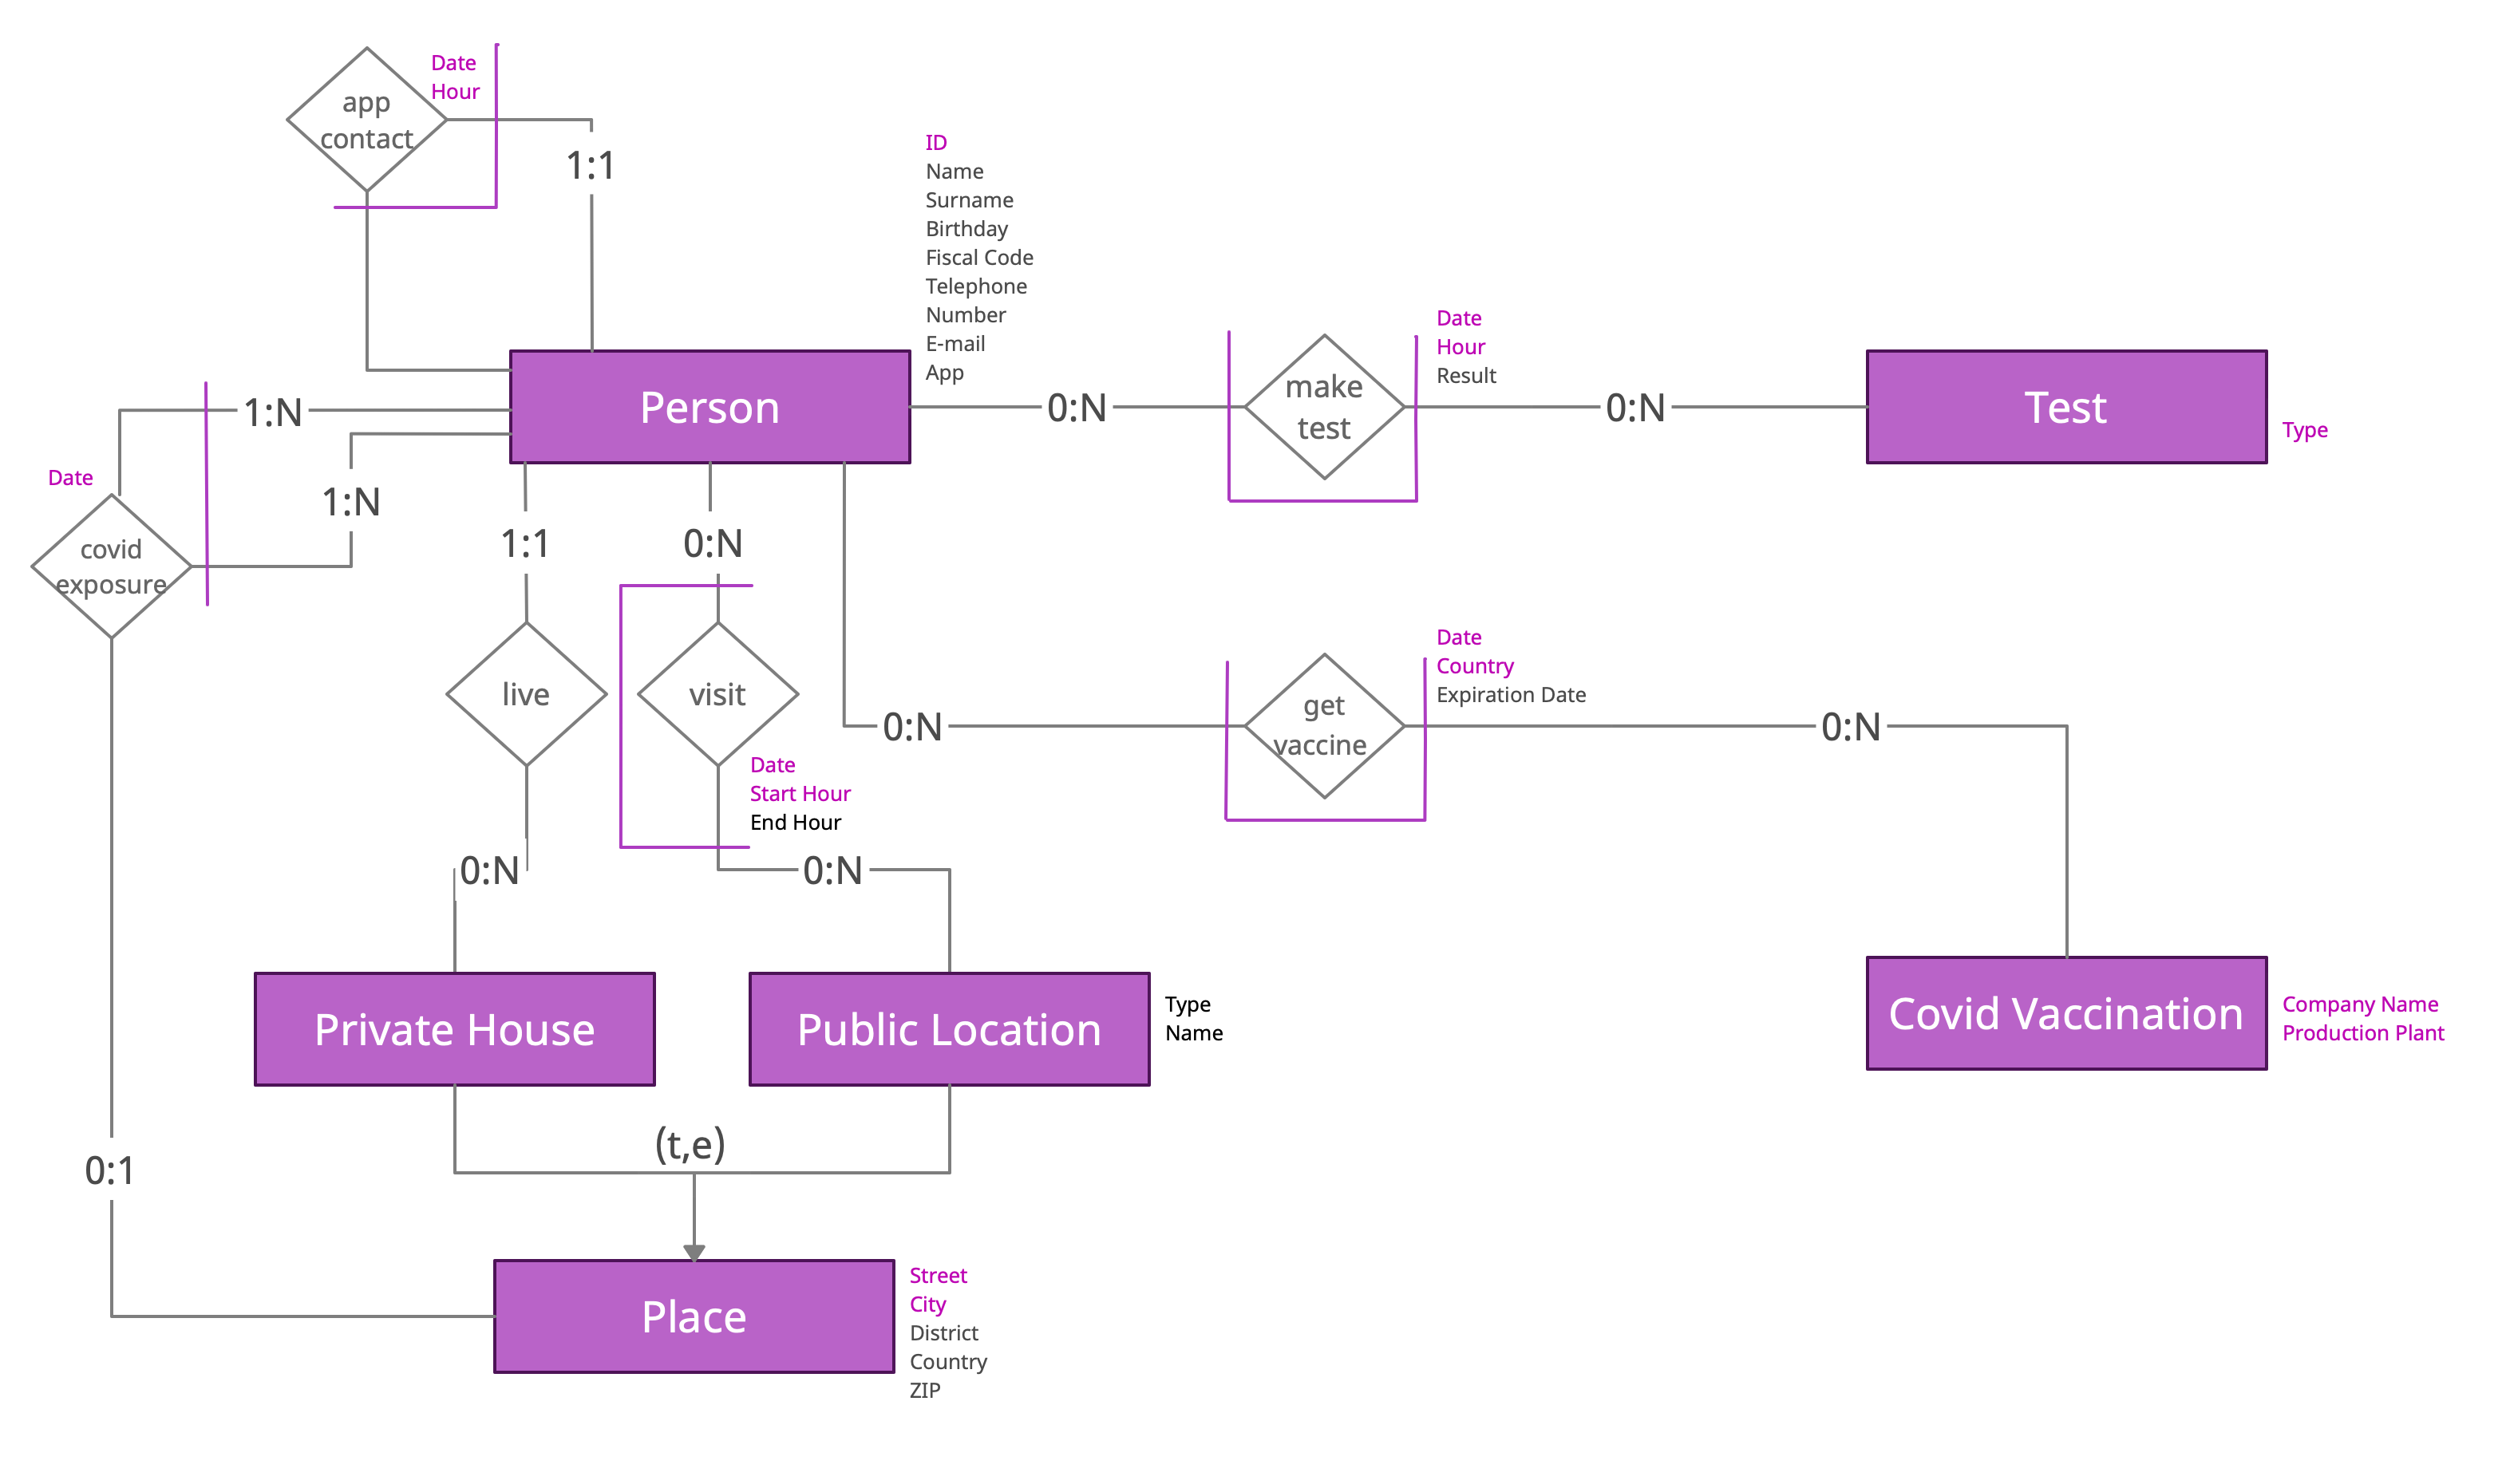
\includegraphics[width=0.8\paperwidth]{images/ImmunoPoli-ER.jpg}
    }
\caption{\textit{Entity Relationship model}}
\end{figure}

\subsection{Entities}
\begin{itemize}
    \item \textbf{Person:} man or woman identified by a unique ID. The ID is also the key for logging into the app. The property \textit{app} is a boolean attribute used to identify whether or not the person has any type of contact tracing application.
    \item \textbf{Place:} general concept of place characterized by an address.
    \item \textbf{Private house:} place that hosts either a group of flatmates or a family. The name of the house corresponds to the owner's name and surname. 
    \item \textbf{Public place:} represents indoor places accessible providing personal information for traceability purposes.
    \item \textbf{Covid Vaccination:} the COVID-19 vaccines. 
    They are identified through their company name and the production plant from where they come.
    \item \textbf{Test:} the COVID-19 tests. They are identified through their class. The distinction is between the tests that detect the viral presence through the \textit{PCR}, \textit{Molecular}, \textit{Antibody} (to check the presence of the virus antagonists) and in the end, the \textit{Rapid} ones. 
\end{itemize}

\subsection{Relationships}
\begin{itemize}
    \item The \textit{\textbf{covid exposure}} relationship represents a \emph{possible viral infection}. Once a positive test is inserted into the database, the system triggers a command\footnote{see section \ref{section: 6} for further details about the command.} to easily find all the people at risk of contagion and notify them of the possible infection. People are obliged to make a swab, and in case of a negative result after at least seven days, the relationship is deleted.
    \item The \textit{\textbf{live}} relationship binds a person with where he resides.
    \item The \textit{\textbf{visit}} relationship involves all the public places where it is more likely that personal information is collected. It serves both realism and simplicity purposes because we don't need to take care of outdoor spots.
    \item The \textit{\textbf{app contact}} relationship gathers all contacts detected by any tracking system that supports localization and applications installation, regardless of its type.
    \item The \textit{\textbf{make test}} relationship links the user with a tests he has made. It contains information such as the hour, the date and the outcome.
    \item The \textit{\textbf{get vaccine}} relationship connects the user to the vaccine he got. As well as \emph{make test}, it is characterized by the date and hour of the injection.
\end{itemize}
\newpage
\section{Dataset description}
\label{section: 4}
The dataset is drawn from a random generator. It allows enforcing parameters such as the number of visits, tests, covid vaccinations, families and the probability of being positive. \\
The generator sequentially builds the graph starting from people, places, families and groups of flatmates. \\
Families are sets of people with at most two different surnames, whereas flatmates are combined randomly. \\
Afterwards, it adds all the vaccinations ensuring that the first dose of vaccine grants a one-month validity certification. The second vaccination provides one-year validity certification employing the same vaccine as the first one. \\
Then, it builds instances of \textit{make test} relationships. 
Every time a positivity status is confirmed, we check the previous contacts and the visited places to look for any \textit{covid exposure} relationships. Moreover,  to ensure the assumption in section 2.\ref{assumption_2}, those who have been tested positive are prevented from going out from then on.

\section{Queries}
\begin{enumerate}[leftmargin=*,label=\textbf{\thesection.\arabic*}]
\item Find undirected contacts stored in the \textit{app contact} relationship.
\begin{figure}[h]
    \centering
    
\includegraphics[width=\textwidth]{images/find_indirected_app_contacts.png}
\end{figure} 
\item Find the mean age of the infected\footnote{We refer to infected people as the positive-tested in the last ten days.} people in the last ten days.
\begin{figure}[h]
    \centering
    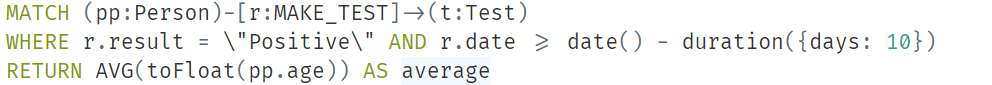
\includegraphics[width=\textwidth]{images/mea_age_last_days.png}
\end{figure} 
\item Find people that live with someone who has been tested positive in the last ten days.
\begin{figure}[h]
    \centering
    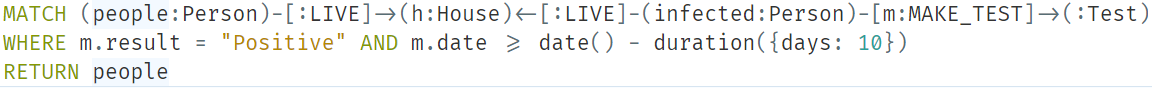
\includegraphics[width=\textwidth]{images/mates_of_positive.png}
\end{figure} 
\item Find the homes where resides someone tested positive in the last ten days.
\item Find the number of test performed in the last month.
    \item Find the number of infected people in a given month.
    \item Find the number of vaccinations performed in a given month.
    \item Find the number of people with a single vaccine dose in a given CAP.
    \item Find the number of people vaccinated in a given CAP.
    \item Find the first five places according to the rate of positive people in the last month.
    \item Find the people exposed to the virus who have not been tested yet.\footnote{They haven't made a swab from the date of the last covid exposure until now.} 
    \item Find the percentage of infected people that got at least one dose of vaccine.
\end{enumerate}

\newpage
\section{Commands}

\section{Application}
The application is the database entry point, and it is projected to be run either by a a government employee or a generic user. The starting page shows the two possible ways to access it.
\begin{figure}[h]
    \centering
    \begin{minipage}{0.475\textwidth}
        \centering
        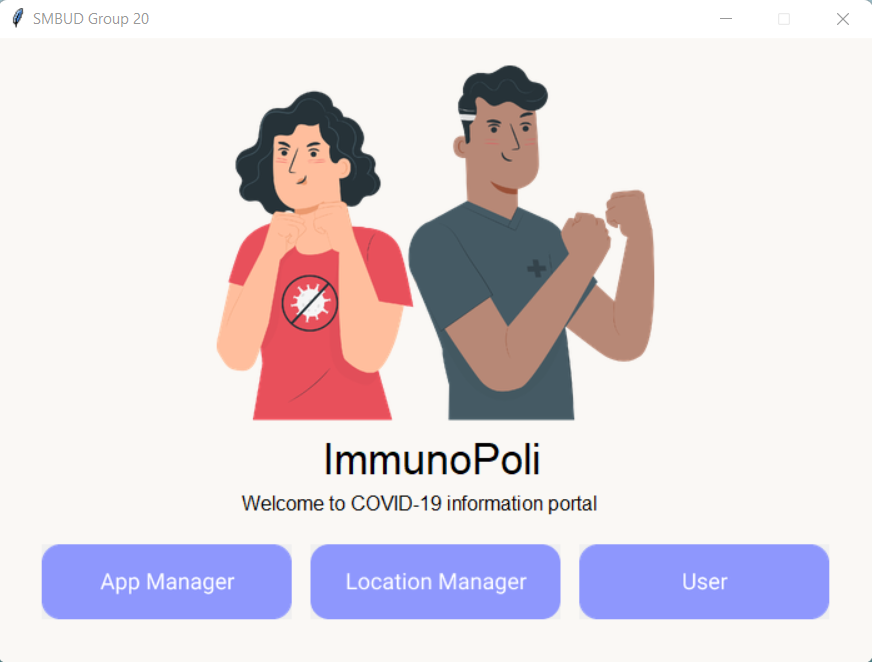
\includegraphics[width=\textwidth]{images/starting_page.png} 
        \caption{\textit{starting page}}
        \label{figure 2}
    \end{minipage}\hfill
    \begin{minipage}{0.475\textwidth}
        \centering
        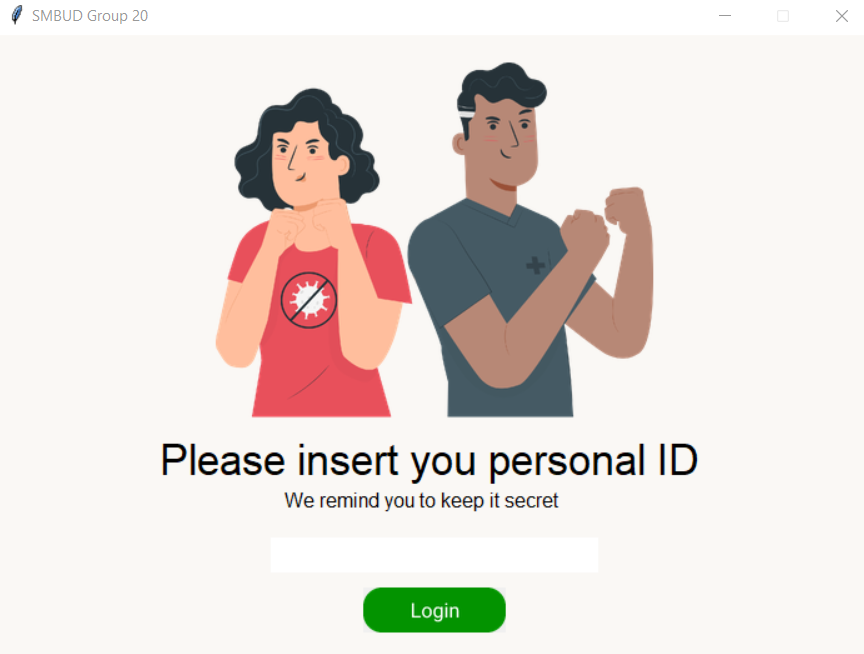
\includegraphics[width=\textwidth]{images/login_page.png} 
        \caption{\textit{login page}}
        \label{figure 3}
    \end{minipage}
\end{figure}
\newline
The first category of users has access to two features:
\begin{itemize}
    \item changing his/her personal information;
    \item examining the places he has visited and the risk he linked to them;
    \item checking his covid exposures;
    \item seeing the history of his tests and related outcomes.
\end{itemize}
The second category instead, has full access to the features:
\begin{itemize}
    \item adding information concerning COVID tests;
    \item monitoring COVID trends;
\end{itemize}


\end{document}